\documentclass[11pt,a4paper]{article}
\usepackage[T1]{fontenc}
\usepackage{lmodern,microtype,amsmath,amssymb,amsthm,booktabs}
\usepackage[margin=27mm]{geometry}
\usepackage{tikz,hyperref,float}
\usetikzlibrary{arrows.meta,positioning,calc}
\hypersetup{colorlinks=true,urlcolor=blue,linkcolor=black,citecolor=black}
\emergencystretch=3em
\newtheorem{theorem}{Theorem}
\newtheorem{lemma}[theorem]{Lemma}
\newtheorem{proposition}[theorem]{Proposition}
\newcommand{\PalomarEntry}{\textsf{Registration pending; URL to be inserted after confirmation}}
\newcommand{\Gcoords}{%
\coordinate (v0) at (-2.8,0);\coordinate (v3) at (-.8,0);
\coordinate (v5) at (-1.8,1.2);\coordinate (v6) at (-1.8,-1.2);
\coordinate (v1) at (2.6,0);\coordinate (v4) at (4.6,0);
\coordinate (v7) at (3.6,1.2);\coordinate (v8) at (3.6,-1.2);
\coordinate (v2) at (.9,-2.5);}
\newcommand{\Gedges}{\foreach \a/\b in {0/3,0/5,0/6,1/4,1/7,1/8,2/6,2/8,3/5,3/6,4/7,4/8,5/7,6/8}{\draw[line width=.7pt] (v\a)--(v\b);}}
\newcommand{\Gvertices}{\foreach \i in {0,1,2,3,4,5,6,7,8}{\node[draw,fill=white,circle,inner sep=0pt,minimum size=7mm,font=\small\bfseries] at (v\i) {\i};}}
\title{A Nine-Vertex Counterexample to the Critical Almost Stacked Hypothesis}
\author{John Fairfax-Ball}
\date{18 October 2026 \quad Working draft, not submitted}
\begin{document}
\maketitle
\begin{abstract}
We give a nine-vertex connected non-bipartite graph disproving both the stacking and clearing clauses of the intended critical Almost Stacked Hypothesis of Csern\'ak and Soukup. The graph has stacking and clearing numbers equal to \(15\), but every almost stacked configuration of size at least \(14\) succeeds. The only losing size-\(14\) configurations are a pair of non-almost-stacked automorphic images. The finite statement has separate Lean kernel-checked losing-layer certificates for both games. We expose the recursion and checker correctness underlying the computer-assisted proof.
\end{abstract}
\section{Introduction}
Csern\'ak and Soukup introduced the stacking and clearing numbers of graphs and proposed the Almost Stacked Hypothesis (ASH) as a possible analogue of a cover-pebbling phenomenon \cite{CSApril,CSOctober}. A crucial distinction is between the \emph{printed, pointwise} least-exact-size hypothesis and the \emph{critical} version ASH$^*$ comparing largest losing layers. A personal clarification from an original author, recorded in the project history, identifies the critical version as intended. We do not claim a published correction or endorsement. We refute the critical form itself, simultaneously for both operations. The earlier tree stacking formula \cite{TreeStack} is a separate result, not an ingredient.
\begin{theorem}[Double counterexample]\label{thm:main}
Let \(G_9\) be the graph on \(\{0,\ldots,8\}\) with the fourteen edges
\[
\{03,05,06,14,17,18,26,28,35,36,47,48,57,68\}.
\]
Its graph6 code is \texttt{HCQTaXi}. It is connected and non-bipartite. Both stacking and clearing have guaranteed threshold \(15\), and in both games the largest losing mass is \(L_{\mathrm{all}}=14\) while the largest almost-stacked losing mass is \(L_{\mathrm{AS}}=13\). The \emph{only} mass-\(14\) losers are
\[
c^*=(0,0,1,0,0,5,0,8,0),\quad c^{*\prime}=(0,0,1,0,0,8,0,5,0).
\]
Neither is almost stacked, hence both universal critical clauses ASH$^*$ are false.
\end{theorem}
\begin{figure}[H]\centering
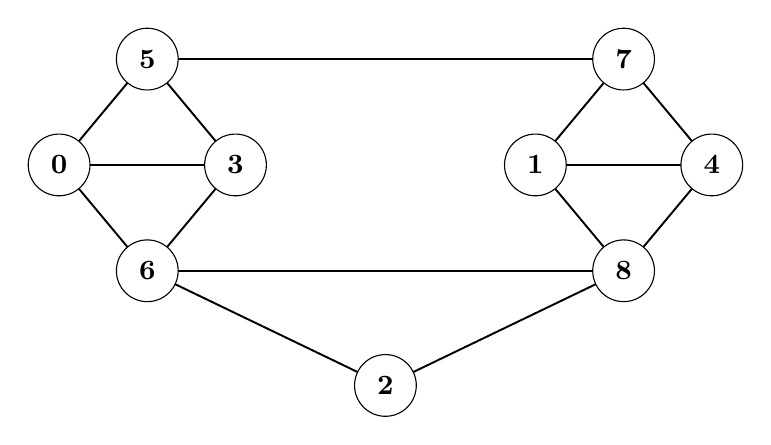
\begin{tikzpicture}[scale=1.12,every node/.style={transform shape}]
\Gcoords\Gedges\Gvertices
\end{tikzpicture}
\caption{\(G_9\): its nine labelled vertices and exactly fourteen edges, with graph6 \texttt{HCQTaXi}. The diamond units have bridges \(5\)--\(7\) and \(6\)--\(8\); vertex \(2\) joins \(6\) and \(8\). Edge fidelity is mechanically checked by \texttt{figure\_check.py}.}\label{fig:g9}
\end{figure}
\section{Definitions and conventions}
A configuration is a vector \(c:V(G)\to\mathbb{N}_0\) of total mass \(|c|=\sum_v c(v)\). One pebbling move \(u\to v\) requires an edge \(uv\) and \(c(u)\ge2\), replaces \(c\) by \(c-2e_u+e_v\), and lowers the mass by one. A configuration is \emph{stackable} if a finite sequence (possibly empty) ends with precisely one occupied vertex; it is \emph{clearable} if such a sequence ends with mass exactly one. Clearability implies stackability. The parameters \(\operatorname{stack}(G)\), for connected graphs with at least two vertices, and \(\operatorname{clear}(G)\), for connected non-bipartite graphs, are the least \(t\ge2\) for which \emph{every configuration of size exactly \(t\)} wins \cite{CSApril}.
A configuration is \emph{almost stacked} (AS) when some root \(r\) satisfies \(c(v)\le1\) for every \(v\ne r\). For each game \(P\in\{\mathrm{stack},\mathrm{clear}\}\) denote the losing configurations of mass \(t\) by \(\mathcal{L}_t^P\). Set
\begin{align*}
L_{\mathrm{all}}^P&=\max\{t\ge2:\mathcal{L}_t^P\ne\varnothing\},\\
L_{\mathrm{AS}}^P&=\max\{t\ge2:\mathcal{L}_t^P\text{ contains an AS input}\}.
\end{align*}
The critical form ASH$^*$ says the universal threshold equals the least \(t_0\ge2\) for which \emph{every almost stacked configuration of every size \(s\ge t_0\)} wins. Equivalently \(L_{\mathrm{all}}^P=L_{\mathrm{AS}}^P\) in the graph classes above. This is not the stronger printed \emph{least exact \(t\)} statement.
\begin{figure}[H]\centering
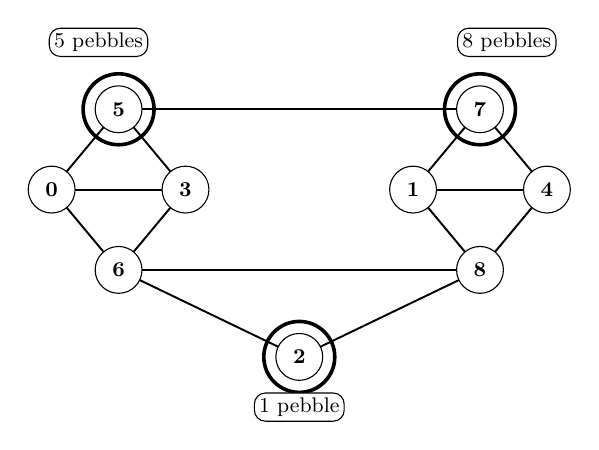
\begin{tikzpicture}[scale=.85,every node/.style={transform shape}]
\Gcoords\Gedges\Gvertices
\foreach \i in {2,5,7}{\draw[line width=1.3pt] (v\i) circle (5.3mm);}
\node[draw,fill=white,rounded corners,inner sep=2pt,font=\small] at ($(v5)+(-.3,1)$) {5 pebbles};
\node[draw,fill=white,rounded corners,inner sep=2pt,font=\small] at ($(v7)+(.4,1)$) {8 pebbles};
\node[draw,fill=white,rounded corners,inner sep=2pt,font=\small] at ($(v2)+(0,-.75)$) {1 pebble};
\end{tikzpicture}
\caption{The critical loser \(c^*\) has \(1+5+8=14\) pebbles, on vertices \(2,5,7\). Double-rimmed vertices are occupied; all others have zero. It is not AS, since \(5\) and \(7\) both have multiple pebbles. The automorphism \((0\,1)(3\,4)(5\,7)(6\,8)\) yields the other loser.}\label{fig:loser}
\end{figure}
\section{Losing-layer recurrence and finite proof}
For either game, mass one is winning, so \(\mathcal{L}_1^P=\varnothing\). Every move reduces mass by one; thus, for \(t\ge2\),
\begin{equation}\label{eq:rec}
c\in\mathcal{L}_t^P\iff |c|=t\text{ and every legal successor of }c\text{ lies in }\mathcal{L}_{t-1}^P.
\end{equation}
This is a precise equivalence, including no-move losses. Every loser is a 0--1 vector or is obtained by reversing a move from the previous losing layer. Therefore the complete candidate set can be chosen as
\begin{equation}\label{eq:candidate}
\begin{aligned}
\mathcal C_t^P={}&\{c\in\{0,1\}^{V}:|c|=t\}\\
&{}\cup\{s+2e_u-e_v:s\in\mathcal L_{t-1}^P,\ uv\in E,\ s(v)\ge1\}.
\end{aligned}
\end{equation}
Formula \eqref{eq:rec} retains exactly the losing members of \eqref{eq:candidate}. For an arbitrary losing \(c\) with a move \(u\to v\), its successor is necessarily losing by \eqref{eq:rec}, and reversing the move recovers \(c\). If there is no move then every coordinate is at most one on a graph without isolated vertices. Thus candidate completeness and soundness do not assume the result.
\begin{proposition}[Certified finite ingredients]\label{prop:cert}
In each of STACK and CLEAR on \(G_9\):
\(\mathcal L_{14}=\{c^*,c^{*\prime}\}\), \(\mathcal L_{15}=\varnothing\),
each layer \(2\le t\le14\) is nonempty, and
\(w=(0,0,1,0,1,11,0,0,0)\) is an AS loser of mass \(13\).
\end{proposition}
\begin{proof}[Computer-assisted, Lean kernel-checked]
The Lean development defines the legal-move reflexive-transitive reachability predicate and the separate STACK and CLEAR goals in \path{formal/AlmostStacked/Defs.lean}. Its \texttt{Checker.lean} proves that an encoded ordered losing-layer tree matches the mathematical losing predicate using the successor equation, ordered-tree membership, goal exclusion and a formally proved candidate-completeness condition. The data arrays are untrusted generated candidates. Each Boolean finite-layer condition is evaluated inside the Lean kernel with \texttt{decide +kernel}; the chain of layers \(2,\ldots,15\) is checked separately for STACK and CLEAR. The exact size-\(14\) characterisation, size-\(15\) emptiness, \(w\), and all lower-layer witnesses are proved in \path{formal/AlmostStacked/Main.lean}. No claim of hand enumeration is made.
\end{proof}
\begin{table}[H]\centering\small
\begin{tabular}{r rr@{\quad}r rr}\toprule
Mass & STACK & CLEAR & Mass & STACK & CLEAR\\\midrule
2&36&36&9&2510&2510\\
3&128&137&10&1301&1301\\
4&383&384&11&473&473\\
5&930&932&12&124&124\\
6&1862&1863&13&21&21\\
7&2887&2887&14&2&2\\
8&3280&3280&15&0&0\\\bottomrule
\end{tabular}
\caption{Exact number of losing configurations at each mass; recorded as cold-rechecked finite layers. These are not estimates.}\label{tab:counts}
\end{table}
\begin{lemma}[Monotonicity above the order]\label{lem:monotonic}
If \(G\) has \(n\) vertices and no isolated vertices and all configurations of mass \(t\ge n\) win a given goal (STACK or CLEAR), then every configuration of every mass \(s\ge t\) wins.
\end{lemma}
\begin{proof}
If \(s>t\ge n\), the pigeonhole principle gives a vertex holding at least two pebbles. Move once along an incident edge; the resulting mass is \(s-1\). Descending induction finishes.
\end{proof}
\begin{proof}[Proof of Theorem~\ref{thm:main}]
The graph is connected by inspection of its listed edges, and has the odd triangle \(0,3,5\). The certificate proposition gives all-size-\(15\) success; Lemma~\ref{lem:monotonic} propagates it above \(15\). The nonempty layers \(2,\ldots,14\) establish the least guaranteed exact threshold \(15\). At mass \(14\), the two losers both have two occupied vertices with at least two pebbles. Thus no AS input loses at \(14\); every larger input wins; and the specified AS input \(w\) loses at \(13\). Hence \(L_{\rm AS}=13\), \(L_{\rm all}=14\) for both games. This refutes the two critical universal clauses.
\end{proof}
\begin{figure}[H]\centering
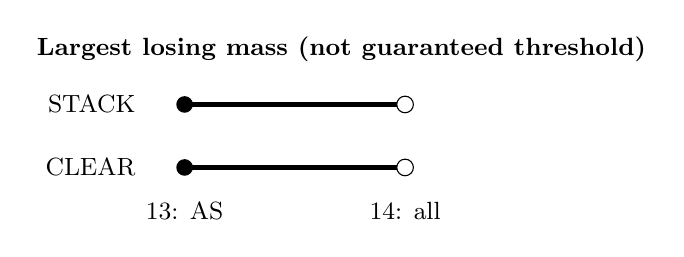
\begin{tikzpicture}
\node[anchor=west,font=\small\bfseries] at (0,2.15) {Largest losing mass (not guaranteed threshold)};
\foreach \y/\lab in {1.45/STACK,.65/CLEAR}{
\node[anchor=east,font=\small] at (1.5,\y) {\lab};
\draw[line width=2pt] (2,\y)--(4.8,\y);
\fill (2,\y) circle (3pt);
\draw[fill=white] (4.8,\y) circle (3pt);}
\node[font=\small] at (2,.1) {13: AS};
\node[font=\small] at (4.8,.1) {14: all};
\end{tikzpicture}
\caption{The sharp gap, identical for STACK and CLEAR: \(L_{\rm AS}=13<L_{\rm all}=14\). In contrast, the \emph{guaranteed thresholds} are respectively \(14\) (AS inputs) and \(15\) (all inputs).}\label{fig:gap}
\end{figure}
\section{Trust boundary and limitations}
The formal target file \texttt{formal/Challenge.lean} specifies twenty-five results, including graph properties, the two mass-\(14\) characterisations, thresholds and both universal negations. The checked theorems use Lean 4.35.0 and Mathlib v4.35.0. Local build and kernel replays were recorded in S017--S019. The S019 fresh-clone test produced a successful plain build and unsandboxed comparator; several independent kernels accepted the export. This is not a hosted Palomar registration or a claim about sandboxed Palomar execution \cite{Repo}.
\begin{figure}[H]\centering
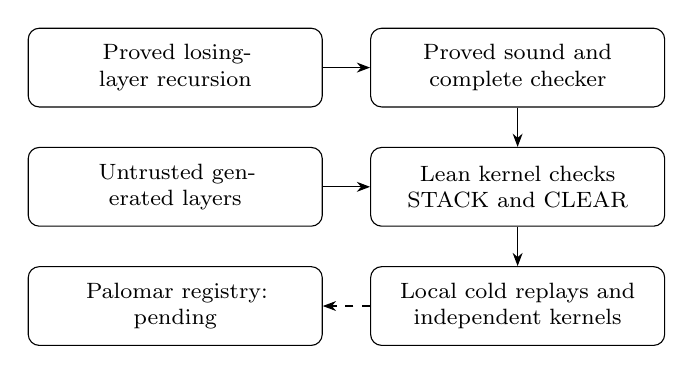
\begin{tikzpicture}[node distance=5mm and 6mm,>=Stealth, bx/.style={draw,rounded corners,text width=35mm,minimum height=10mm,align=center,font=\footnotesize}]
\node[bx] (math) {Proved losing-layer recursion};
\node[bx,right=of math] (checker) {Proved sound and complete checker};
\node[bx,below=of math] (data) {Untrusted generated layers};
\node[bx,right=of data] (lean) {Lean kernel checks\\STACK and CLEAR};
\node[bx,below=of lean] (ind) {Local cold replays and independent kernels};
\node[bx,left=of ind] (pal) {Palomar registry:\\pending};
\draw[->] (math)--(checker);\draw[->](checker)--(lean);\draw[->](data)--(lean);
\draw[->](lean)--(ind);\draw[->,dashed](ind)--(pal);
\end{tikzpicture}
\caption{Formal verification architecture. The dashed last step is pending; the Palomar service is not represented as having accepted the package.}\label{fig:verification}
\end{figure}
An order-\(9\) witness does not prove uniqueness in the class of all order-\(9\) graphs, given outstanding independently unverified atlas cases. The suggested infinite bridge families remain conjectural. Novelty audits at two phases were waived by the owner, not passed; no global priority claim is made. The earlier tree stacking theorem \cite{TreeStack} is acknowledged as independent prior work.
\section*{Availability, acknowledgements and declarations}
Source: \url{https://github.com/jfairfaxball-348/Almost-Stacked-Proof}. Exact Lean submission snapshot (distinct from research main): \texttt{palomar/submission}, commit \texttt{34363e5222136c54}\allowbreak\texttt{b08e0c5550e2d49b9f23f5fd}. Palomar verification: \PalomarEntry. To regenerate diagrams and check graph integrity run \texttt{python3 figure\_check.py}; build commands and environment are in \texttt{paper/README.md}. No external registration, journal/arXiv submission or email is made here. The pebbling parameters and motivating conjecture are due to Tam\'as Csern\'ak and Lajos Soukup \cite{CSApril,CSOctober}. Computational, formal and drafting assistance was used; the named author remains responsible for the paper.
\bibliographystyle{plain}
\bibliography{references}
\end{document}
